\documentclass[12pt]{article}
	
\usepackage[margin=1in]{geometry}		% For setting margins
\usepackage{amsmath}				% For Math
\usepackage{fancyhdr}				% For fancy header/footer
\usepackage{graphicx}				% For including figure/image
\usepackage{cancel}					% To use the slash to cancel out stuff in work

%%%%%%%%%%%%%%%%%%%%%%
% Set up fancy header/footer
\pagestyle{fancy}
\fancyhead[LO,L]{Chengming Li}
\fancyhead[CO,C]{ECE257a - Homework2}
\fancyhead[RO,R]{\today}
\fancyfoot[LO,L]{}
\fancyfoot[CO,C]{\thepage}
\fancyfoot[RO,R]{}
\renewcommand{\headrulewidth}{0.4pt}
\renewcommand{\footrulewidth}{0.4pt}
%%%%%%%%%%%%%%%%%%%%%%

\begin{document}

\noindent \textbf{Problem 1 (16pt). True or false questions. If false, explain why\\}


\begin{enumerate}
\item  With Nt transmit antennas, closed-loop MIMO can increase the link capacity by Nt times
compared with SISO.\\
\textbf{Answer}: False, Based on $C = Blog_2(1+SNR)$, Nt transmit antennas would only increase the link capacity by $log_2(Nt)$ times
\item  MU-MIMO requires time, frequency and phase synchronization between different receivers.\\
\textbf{Answer}: False, not the receiver, it is the transmitter 
\item  MU-MIMO can scale network capacity linearly with the number of transmitters.\\
\textbf{Answer}: False, in general, capacity gain from spatial multiplexing scales linearly with $min(N_t,N_r)$

\item  Channel partitioning MAC has higher efficiency than random access MAC because the
former doesn’t have to waste time on carrier sensing or random backoff\\
\textbf{Answer}: False, In TDMA unused slots go idle, and the time is wasted. Same in FDMA, unused transmission time in frequency bands go idle.
\item  In pure ALOHA, a node does not need a local clock. So pure ALOHA is much simpler than
slotted ALOHA\\
\textbf{Answer}: True

\item  In 802.11 CSMA/CA, during backoff, a node needs to freeze its timer if the channel becomes
busy again\\
\textbf{Answer}: True
\item  In 802.11 CSMA/CA, a transmitter’s backoff counter is doubled if it doesn’t hear an ACK
confirmation from the receiver after a transmission.\\
\textbf{Answer}: False, if no ACK, increase random backoff interval, not double.
\item  A WiFi access point can be considered a router running IP routing protocols. \\
\textbf{Answer}: False, WIFI ap and router are two different devices. WIFI AP doesn't need to perform IP routing, while Router does. Router connects different IPs. In real life, they usually combine into one unit.
\end{enumerate}
	

		
\noindent \textbf{Problem 2 (26pt). Understand MIMO gains.\\}
\begin{enumerate}
\item  (10pt) Explain the asymptotic gains from the following 4 MIMO schemes: receiver diversity,
open-loop transmit diversity, closed-look transmit diversity, spatial multiplexing, and multi-user
MIMO. In particular, explain how the MIMO capacity increases with the number of antennas,
and intuitively why. Review the lecture notes and references, and provide the answers based on
your own understanding.\\
\textbf{Answer}: receiver diversity: Increasing SNR proportionally to $N_r$(number of receiving antennas), The received signal power just adds up. Based on the equations from lecture notes, the combined SNR is $SNR = \frac{N_r * |h|^{2}}{\sigma^{2}}$. So when the SNR is low, the gain is almost linear w.r.t.Nr. When SNR is high, gain is approximately $log(N_r)$\\\\
\textbf{Answer}: open-loop transmit diversity: It causes the received SNR to "harden" to the average SNR. In other words, it iliminates the effects pf small-scale fading but does not increase the average received SNR. Based on the equation from lecture notes, $SNR = \frac{\epsilon}{\sigma^{2}} * E[h_1]^{2}$\\\\
\textbf{Answer}: closed-look transmit diversity: With $N_t$ TX antennas, SNR increases to $N_t$ times, assuming total transmit power remains constant. And based on Shannon's equation, the gain is $C = Blog_2*(1+SNR)$. So the gain is linear as $log_2(SNR)$\\\\
\textbf{Answer}: spatial multiplexing: In general, capacity gain from spatial multiplexing scalies linearly with $min(N_t, N_r)$. Since base on the "system of equations" model, $N_t$ determines the number of variables, and $N_r$ determines the number of eqns.\\\\
\textbf{Answer}: multi-user MIMO: If the transmitter has $N_t$ antennas, then it can send $N_t$ streams of data simultaneously to $N_t$ users, increasing capacity to $N_t$ times compared with single-antenna transmitter.\\\\

\item  (8pt) Compare two networks: a single-user MIMO network with one 4-antenna transmitter
and one 4-antenna receiver, versus a MU-MIMO network with 4-antenna access point and 4
single-antenna users. Suppose the channel matrices are the same for these two setups. Will thetwo networks have the same total throughput? Why? (Note: Here we count the net throughput,
not bit-rate. So transmission overhead matters.).\\
\textbf{Answer}: No they won't have the smae total throughput, In the case of a single-user MIMO 4*4, the throughput gain is linearly with 4. But in the case of MU-MIMO 4*4, the MU-MIMO requires closed-loop, non-trivial oberhead, making the net throughput gain lower than $N_t$ time, which is less than 4. So, they don't have the same total throughput.\\\\

\item  (8pt) Consider a 2x2 MIMO link, if both transmitter’s antennas are placed very close to eachother, and receiver’s antennas are also close to each other, then the spatial multiplexing gain maybe low due to channel correlations of nearby antennas.What if we separate the receiver’s antennas far enough away from each other, but keep the transmitter’s antennas close to each other? (Hint: Think of the problem of achieving multiplexing gain as the problem of solving a system of equations)
In this case, will the link still likely have higher capacity than SISO? (Hint: Can there be any diversity gain?)\\
\textbf{Answer}: It's still likely to have higher capacity than SISO, because the receiver's antennas are separated far enough away from each other. So it's like a SIMO that we can get the receiver diversity from this setup. And asymptotic gain is proportionally to $N_r$.
And the equations we can get is, $y_1 = h_{11}*x_1$ and $y_2 = h_{21}*x_1$
\end{enumerate}

\noindent \textbf{Problem 3 (15pt). Understand the working principle of MU-MIMO.\\}
\begin{enumerate}
\item  Consider the following MU-MIMO scenario: a single 3-antenna transmitter (TX) is
transmitting data to 3 single-antenna users RX1, RX2, and RX3 simultaneously. Suppose the
channel gain values hij are known to the TX. Suppose the transmitter wants to ensure RX1
receivers a symbol x, but RX2 and RX3 hear nothing (essentially they hear 0, or a null value).
Then what should each of the 3 transmit antennas send? (Hint: Construct a system of equations
and solve it.)\\
\textbf{Answer}: Solved by MatLab\\\\
$\begin{array}{l}
\left(\begin{array}{c}
\frac{h_{22} \,h_{33} \,x-h_{23} \,h_{32} \,x}{\sigma_1 }\\
-\frac{x\,{\left(h_{21} \,h_{33} -h_{23} \,h_{31} \right)}}{\sigma_1 }\\
\frac{x\,{\left(h_{21} \,h_{32} -h_{22} \,h_{31} \right)}}{\sigma_1 }
\end{array}\right)\\
\mathrm{}\\
\textrm{where}\\
\mathrm{}\\
\;\;\sigma_1 =h_{11} \,h_{22} \,h_{33} -h_{11} \,h_{23} \,h_{32} -h_{12} \,h_{21} \,h_{33} +h_{12} \,h_{23} \,h_{31} +h_{13} \,h_{21} \,h_{32} -h_{13} \,h_{22} \,h_{31} 
\end{array}$\\\\
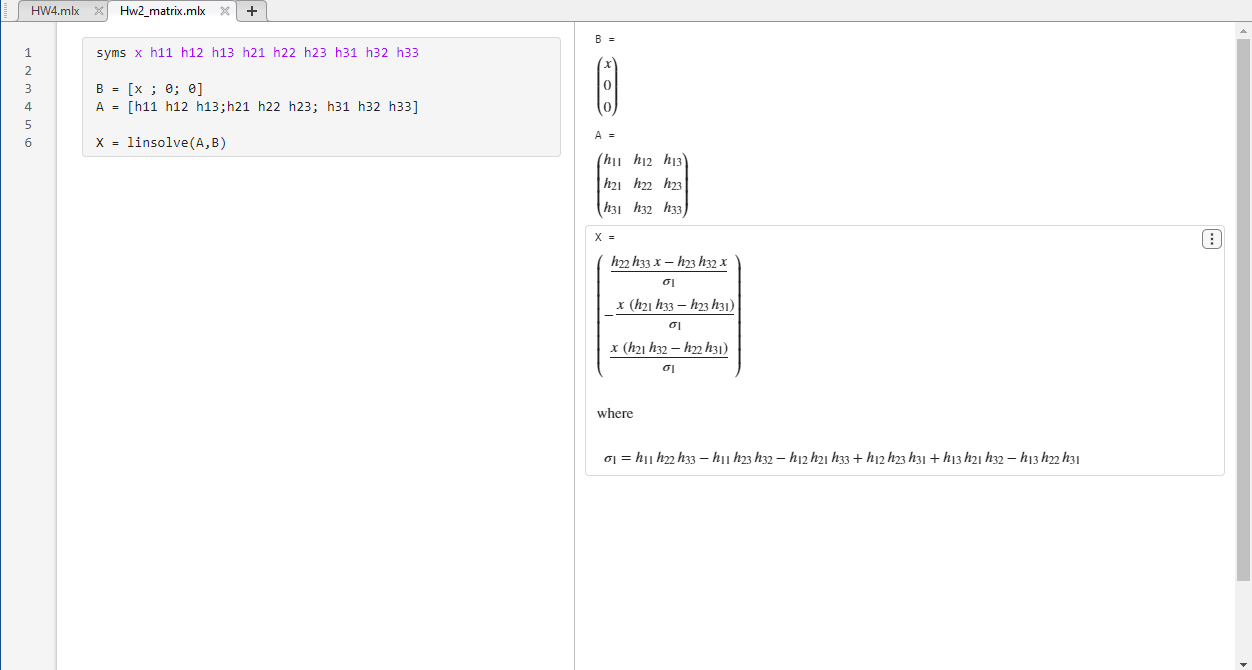
\includegraphics[scale=0.5]{HW4_Q3a).png}\\\\

\item  Consider a MU-MIMO network where a 2-antenna transmitter is transmitting data to 2
single-antenna users RX1 and RX2. Suppose the announcement packet and data packet are 100
Bytes and 1 KB respectively. The CSI feedback packet and ACK packet are 100 Bytes, 100
Bytes for both users. The data packet is sent at 100MBps, and all other packets are sent at
10MBps. Then what is the maximum achievable throughput of the network? \\\\
\textbf{Answer}: The whole process is $Announcement + RX_1 CSI + RX_2 CSI + DATA + ACK_1 + ACK_2$\\
Announcement = $\frac{100}{10M} = 10us$\\
$RX_1 CSI + RX_2 CSI$ = $\frac{100}{10M} *2 = 20us$\\
DATA = $\frac{1K}{100M} = 10us$\\
$ACK_1 + ACK_2 $ = $\frac{100}{10M} *2 = 20us$\\
Total = 60us\\
Throughput = $\frac{1K}{60u} = 16.67 MBps$\\

\end{enumerate}

\noindent \textbf{Problem 4 (16pt). MAC protocols. Summarize the pros and cons of the following MAC protocols: TDMA, FDMA, Polling, Token Rings, Slotted LOHA, pure ALOHA, CSMA/CD.\\}
\textbf{Answer}:\\
TDMA:\\
Pros: Low chance of collisions, simple, and having control of the channel. Easy to predict the behavior\\
Cons: Unused slots go idle. Un-efficiency. Synchronization is required across devices\\

\noindent FDMA:\\
Pros: Low chance of collisions, simple, and having control of the channel. Easy to predict the behavior \\
Cons: Unused transmission time in frequency bands go idle. Adjacent channel effects\\

\noindent Polling:\\
Pros: Low chance of collisions and empty slots.\\
Cons: polling delay and master node failure\\

\noindent Token Rings:\\
Pros: decentralized and highly efficient\\
Cons: the failure of one node can crash the entire channel. Recovery procedure must be invoked if the token is unreleased by some nodes\\

\noindent Slotted ALOHA:\\
Pros: Single active node can continuously transmit at full rate of channel. Simple; highly decentralized: only need to sync each slot\\
Cons: collisions, wasting slots; inefficient collision resolution. idle slots, underutilizing channel. Clock sync is required\\

\noindent pure ALOHA:\\
Pros: simpler, no synchronization, decentralized\\
Cons: efficiency is 50 percent lower compared with slotted aloha. More collisions compared to slotted ALOHA\\

\noindent CSMA/CD:\\
Pros: Collisions detected within short time. Reduce channel wastage\\
Cons: more collision means longer backoff time. Not applicable in wireless communication devices due to half-duplex \\\\

\noindent \textbf{Problem 5 (15pt). Slotted ALOHA with heterogeneous nodes. Consider two nodes, A and B,
that use the slotted ALOHA protocol to contend for a channel. Suppose node A has more data to
transmit than node B, and node A’s retransmission probability pA is greater than node B’s
retransmission probability, pB.\\}
\begin{enumerate}
\item Provide a formula for node A’s average throughput. What is the total efficiency of the
protocol with these two nodes?\\
\textbf{Answer}: A's average throughput = $ TransimissionRate(TR) * T_{FrameDuration}(T)*p_A * (1-p_B)$. Total efficiency = $TransimissionRate * T_{FrameDuration} * p_A * (1-p_B)$ + $TransimissionRate * T_{FrameDuration} * p_B * (1-p_A)$\\
\item If pA $=$ 2 pB, is node A’s average throughput twice as large as that of node B? Why or why not? If not, how can you choose pA and pB to make that happen?\\
\textbf{Answer}: A' throughput = $TR * T * p_A * (1-p_B) = TR * T * (2p_B*(1-pB)) = TR * T * (2p_B-2(p_B)^2)$\\
B's throughtput = $TR * T * p_B * (1-p_A) = TR * T *p_B*(1-2p_B) = TR * T *(p_B - 2(p_B)^2)$\\
\\
node A’s average throughput is not twice as large as that of node B. And the only situation to make that happen is when $p_A = p_B$ so that $TR * T * p_B * (1-p_A) = TR * T * p_A * (1-p_B) = TR*T*p(1-p)$
\item In general, suppose there are N nodes, among which node A has retransmission probability 2p and all other nodes have retransmission probability p. Provide expressions to compute the average throughputs of node A and of any other node.\\
\textbf{Answer}\\
A' throughputs: $TR*T * 2p * (1-p)^{N-1}$\\
Any other node: $TR*T * p*(1-2p)*(1-p)^{N-2}$
\end{enumerate}



\noindent \textbf{Problem 6 (12pt). Understanding CSMA/CA. Answer the following questions:\\}
\begin{enumerate}
\item CSMA/CD is not used in current wireless networks such as WiFi. Suppose WiFi radios
become full-duplex in future, will CSMA/CD work just like in classical Ethernet?
\textbf{Answer}: No, even if the transmitter is full-duplex, what it hears may be different from what the receiver actually experiences. The transmission of WIFI drowns out the ability of the radio to hear a collision.

\item What’s the hidden terminal problem(Client1, AP, Client2) in CSMA/CA? Does RTS/CTS fully solve the problem?\\
\textbf{Answer}:  Hidden terminal problem is when Client 1 and Client 2 cannot hear each other. i.e., their transmissions may overlap with higher probability even if they choose different CW sizes.\\ RTS/CTS does not completely solve the hidden terminal problem. RTSs may still collide with each other. But they're short.

\item What’re the negative impacts of the exposed terminal problem in CSMA/CA? Does
RTS/CTS solve the problem?\\
\textbf{Answer}: Exposed terminal(Client1, AP1, AP2, Client2) problem occurs when carrier sensing prevents neighboring senders from transmitting simultaneously, through they do not interfere with each other's receiver. i.e., AP2 heard AP1 is transmitting and stopping the transmission of Client2. This problem reduces spatial reuse opportunities, i.e., reduces effective total network throughput.\\
The RTS/CTS doesn't solve the problem, and make the communication more aggressive.
\item What’s causing the performance anomaly of 802.11? Explain the difference between time
fairness and packet fairness.\\
\textbf{Answer}: Performance anomaly of 802.11 occurs when the throughput of a node sending at a high rate is degraded by the node sending at a low rate. And the root causes is the 802.11 ensures packet fairness instead of time fairness.\\
Packet fairness: Each STA has an equal probability of winning the contention. i.e., the average number of delivered packets for all nodes are roughly the same.\\
Time fairness: each node occupies roughly the same proportion of channel time.

\end{enumerate}

\end{document}